\section{Последовательность решения задачи многокритериальной оптимизации параметров пневмопривода}\label{ch:ch4/sec1}

Решение задачи многокритериальной оптимизации параметров электропневматического привода осуществляется в соответствии с
предложенной методологией, включающей следующие основные этапы.
На первом этапе производится формализация целевых
функций оптимизации. Вводится вектор критериев качества:
\begin{equation}
\mathbf{J}(\mathbf{p}) = \begin{bmatrix}
J_1(\mathbf{p}) \
J_2(\mathbf{p})
\end{bmatrix} = \begin{bmatrix}
\frac{1}{T}\sum_{i=1}^{4}N_i \
\int_0^T (x_{\text{зад}} - x(t))^2 dt
\end{bmatrix}
\end{equation}
где $\mathbf{p}$ -- вектор оптимизируемых параметров алгоритма управления;
$N_i$ -- количество переключений $i$-го распределителя;
$T$ -- время наблюдения;
$x_{\text{зад}}$ -i заданное положение;
$x(t)$ -- текущее положение штока.

Далее осуществляется определение пространства параметров:
\begin{equation}
\mathbf{p} \in \mathcal{P} = {\mathbf{p} \in \mathbb{R}^d: \mathbf{p}{\text{min}} \leq \mathbf{p} \leq \mathbf{p}{\text{max}}}
\end{equation}
где $d$ -- размерность вектора параметров;
$\mathbf{p}{\text{min}}$, $\mathbf{p}{\text{max}}$ -- векторы минимальных и максимальных значений параметров.

На втором этапе формируется начальная выборка точек в пространстве параметров
методом латинского гиперкуба, обеспечивающим равномерное покрытие области
поиска. Для каждой точки выборки проводится численное моделирование системы и вычисляются значения критериев качества.
Процесс этапа схематически представлен на рисунке \ref{fig:step_2_scheme}.

\begin{figure}[ht]
    \centerfloat{
    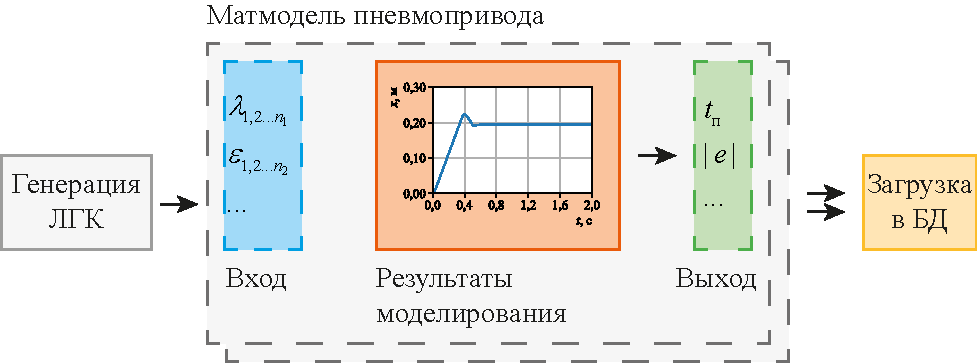
\includegraphics{part4/step_2_scheme.pdf}
    }
    \caption{Схема второго этапа методологии многокритериальной оптимизации.}\label{fig:step_2_scheme}
\end{figure}


Третий этап заключается в построении суррогатных моделей для аппроксимации зависимостей критериев качества от параметров:
\begin{equation}
\hat{J}_i(\mathbf{p}) = f_i(\mathbf{p}, \mathbf{w}_i), \quad i = 1,2
\end{equation}
где $f_i$ -- функция суррогатной модели;
$\mathbf{w}_i$ - вектор параметров модели.

На четвертом этапе осуществляется поиск множества Парето-оптимальных
решений с использованием генетического алгоритма NSGA-II, оперирующего
суррогатными моделями. Фронт Парето формируется как множество недоминируемых решений:
\begin{equation}
\mathcal{P}^* = {\mathbf{p} \in \mathcal{P}: \nexists \mathbf{p}' \in \mathcal{P}, \mathbf{J}(\mathbf{p}') \preceq \mathbf{J}(\mathbf{p})}
\end{equation}

Пятый этап включает верификацию полученных решений путем численного моделирования
системы с выбранными параметрами и уточнение суррогатных моделей в окрестности фронта Парето.

На заключительном этапе производится анализ полученных результатов,
выявление характерных областей фронта Парето и формирование
рекомендаций по выбору параметров алгоритма управления в зависимости от приоритетов между критериями качества.
Предложенная последовательность решения задачи многокритериальной оптимизации
обеспечивает эффективный поиск оптимальных параметров алгоритма
управления электропневматическим приводом с учетом компромисса
между точностью позиционирования и частотой переключений распределителей.

Применение суррогатных моделей позволяет существенно сократить вычислительные затраты при сохранении требуемой точности оптимизации.

Рассмотрим в дальнейшем методы построения суррогатных моделей
и их применение в задаче оптимизации параметров управления пневмоприводом.